\documentclass[uplatex]{jsarticle}
\usepackage[utf8]{inputenc}

\usepackage{amsmath}
\usepackage[dvipdfmx]{graphicx}
\usepackage{resume}  % resume用スタイル
\usepackage{udline}  % 下線用
\usepackage{comment} % 複数行コメント
\pagestyle{plain}
 
\begin{document}
\twocolumn[
    \beginheader{令和5年度 コンピュータサイエンス学部 中中間発表}{2023}{6}{19}{井上 研究室}
    \title{VR環境時の運転シミュレーション酔いの抑制に振動が与える影響}
    \author{C0B20205 武田 夢音 (Yumene Takeda)}
    \endheader
]
\vspace{3mm}

%%ページ番号
\setcounter{page}{9}

\section{はじめに}
近年、VR機器の普及により360度動画の視聴やVRゲームなどのエンターテインメント分野の発展が目覚ましい。これに伴い、子供から高齢者までの幅広い層の使用に耐える品質が求められ、快適性の検討が不可欠となっている。しかし、実際には利用時に違和感を感じたり、眼精疲労、場合によってはめまいや頭痛、吐き気などの「酔い」が起こる問題が生じており、早急な原因究明・対策が望まれている。

酔いの原因については諸説あるが、酔いを良く説明できるものとして感覚不一致説\cite{SensoryConflictTheory}がある。これは、日常の生活で得られる感覚情報パターンは中枢神経内に蓄えられており、船上やVR環境などの普段と異なる感覚情報パターンの環境に置かれた際、中枢神経内で新しい感覚情報パターンへの組み換えが起こると同時に酔いが発生するという説である。

そこで、本研究ではVRを用いないドライビングシミュレータ酔いの抑制に

また逆に,コンテンツを見せるためにウィジェットのサイズを小さくすると,キーの
サイズが大きく下降する.
これらの問題は,ユーザ体験を損なうと同時に,ゲーム内の表現に制限をかけて
いると考えられる.
そこで,入力に必要な負担および画面占有率の低い
文字入力手法を開発するため,2 本のジョイスティッ
クを用いた,フリック入力に基づくかな文字入力手
法 JoyFlick\cite{joyflick},\cite{joyflick_eng}を作製した\footnote{フリック入力に基づく2本の押し込み機能付きジョイスティックを用いたテキスト入力手法. 横山 海青, 髙倉 礼, 志築 文太郎, 川口 一画 Vol.23 No.4, 2021 }.

\begin{figure}[tb]
  % width や height で絶対的な大きさ指定をすることもできる
  \centering
  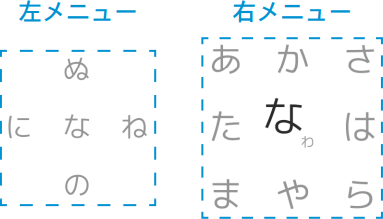
\includegraphics[width=0.7\linewidth]{fig/JoyFlick_menu.png}
  \caption{スティックが全てニュートラルポジションにあるときのJoyFlickのウィジェット}
  \label{fig:JoyFlick}
  \fbox{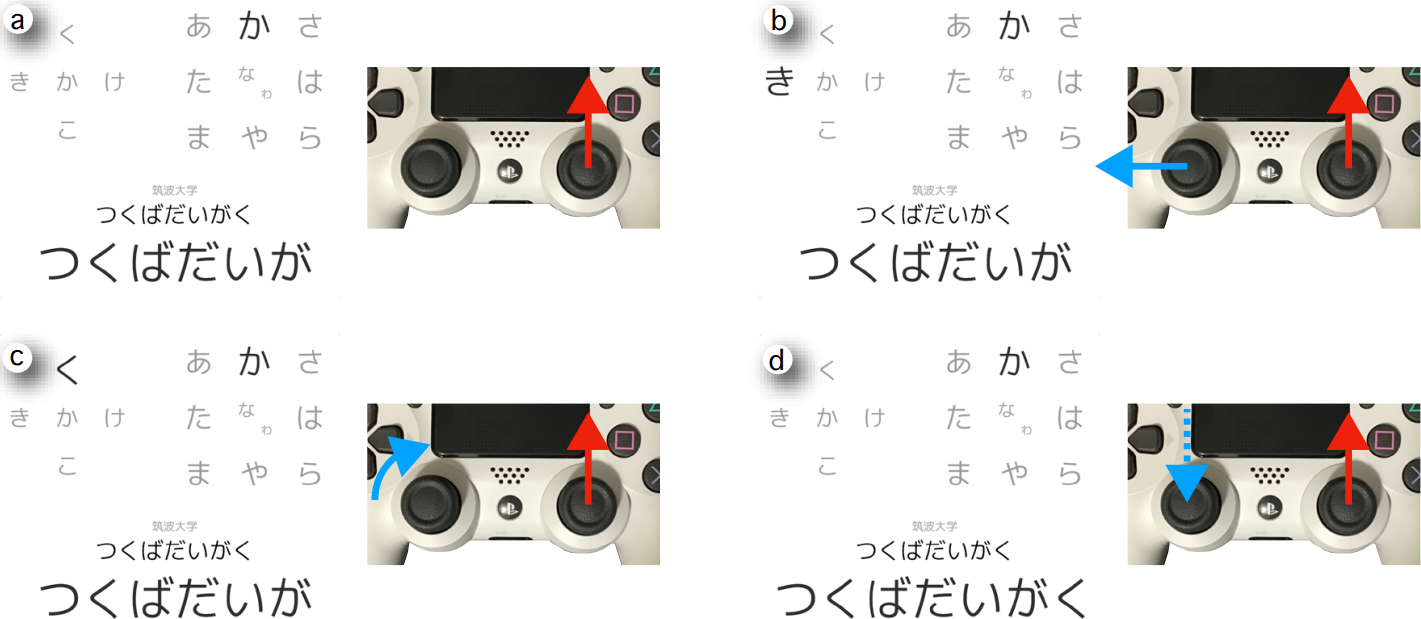
\includegraphics[width=1\linewidth]{fig/JoyFlick_abcd.png}}
  \caption{JoyFlickを用いて「く」を入力する操作の入力例}
  \label{fig:JoyFlick_abcd}
\end{figure}

\section{システム概要}
\subsection{JoyFlick}
\figref{fig:JoyFlick}に示すJoyFlickは押し込み機能付きジョイスティック2つを用いる,フリック入力に基づくかな入力手法である.
JoyFlickは高速なかな文字入力が可能であること,ゲーム機に付随しているデバイスのみを用いること,習得が容易であること,ウィジェットが小さいことを設計の指針としている.

\subsection{操作方法}
ユーザはまず右スティックを用いて\figref{fig:JoyFlick_abcd}のaに示すように子音選択を行い,次に左スティックを用いて\figref{fig:JoyFlick_abcd}のbおよび\figref{fig:JoyFlick_abcd}のcに示すように母音選択を行う.そして最後に,母音選択に用いた左スティックをニュートラルポジションに戻すことにより\figref{fig:JoyFlick_abcd}のdに示すように1文字が入力される.

ユーザは右スティックをニュートラルポジションにすることにより子音「な」,押し込むことにより子音「わ」を選択できる.

Bまたは×ボタンを押すことで最後に入力した文字を消去できる.

\section{実験}
実装にはRust言語を用いて,実験用のアプリケーションをWindows10およびmacOS上に実装した.
実験にはゲームパッドとしてNintendo Switch Proコントローラを用い,ゲームパッドとコンピュータをBluetoothを介して接続した.
まずJoyFlickを初めて使うユーザの入力速度および精度を調べるための初期実験を行った。
その後JoyFlickを継続的に使用し始めたユーザの入力速度および精度を調べるための1週間の長期実験を行った.

\subsection{初期実験}
日本語を母語とする19-25歳の24名が参加した.
参加者はJoyFlickでの入力経験が無く,50音キーボードによる文字入力経験があった.
18名はスマートフォン操作にフリック入力を用いており,残りはQWERTY配列を用いていた.
実験はJoyFlickと50音キーボードの2つの入力方法を用いて行われた.
参加者は2つの入力方法において,28文の計289文字を練習文として入力した後,18文の計168文字を課題文として入力するように求められた.

\subsection{長期実験}
初期実験に参加した参加者から20-25歳の15名が参加し,全て男性であった.
11名はスマートフォンにおいて日頃からフリック入力を用いており,残りはQWERTY配列を用いていた.
実験には初期実験と同じソフトウェアを用い,参加者には課題文の合計が140字を超える直前まで課題文を入力するように求めた.
実験は7日間連続で行われ,参加者は1日にJoyFlickを用いた入力,50音キーボードを用いた入力の合わせて2回を行い,参加者は課題文約18文の平均135文字を入力するように求められた.




\section{結果}
\subsection{初期実験}
入力速度の指標としてCPM(Characters Per Minute)を用いた.JoyFlickおよび50音キーボードの平均入力速度を\figref{fig:res_joy50}に示す.JoyFlickと50音キーボードの平均入力速度はそれぞれ42.8CPMと37.2CPMだった.

\begin{figure}[tb]
  % width や height で絶対的な大きさ指定をすることもできる
  \centering
  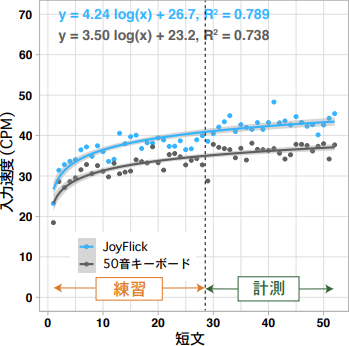
\includegraphics[width=0.7\linewidth]{fig/result_joy50.png}
  \caption{JoyFlickおよび50音キーボードの平均入力速度}
  \label{fig:res_joy50}
  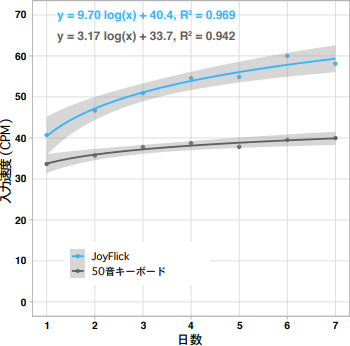
\includegraphics[width=0.7\linewidth]{fig/result_long.png}
  \caption{JoyFlickおよび50音キーボードの平均入力速度}
  \label{fig:res_long}
\end{figure}

\subsection{長期実験}
JoyFlickおよび50音キーボードの平均入力速度を\figref{fig:res_long}に示す.JoyFlickと50音キーボードの平均入力速度はそれぞれ58.1CPMと40.0CPMだった.

\section{まとめ}
本論文では,フリック入力に基づく2本の押し込み機能付きジョイスティックを用いたテキスト入力手法JoyFlickについて述べ,入力速度および精度を評価する実験を行った.
%実験を行う際に,ユーザは文字入力時にスティックを左右ほぼ同時にニュートラルポジションに戻す傾向があることが分かった.
JoyFlickの実用性をさらに示すためには,予測変換と組み合わせる,ゲームに組み込むなどして実際の使用状況に近い環境において入力速度および精度を調査する必要がある.


 \bibliographystyle{junsrt}
\bibliography{ref.bib}   % 参考文献のデータベースファイルを指定する 
\end{document}
